\begin{song}{title=\predtitle\centering Dezolát\\\large Vypsaná Fixa \vspace*{-0.3cm}}  %% sem se napíše jméno songu a autor
\begin{centerjustified}
\nejvetsi

\begin{varwidth}[t]{0.48\textwidth}\setlength{\parindent}{0.45cm}  %Varianta č. 2 --> Dva sloupce

\sloka
	^{Emi\z}Ty~jsi pěkný ^{\,\,C}dezolát,
	
	^*{D}ře kla ,,Halí ^{A}Belí``
	
	a byla to pohoda,
	
	třeba se to povede,
	
	vytáhnem tvý múzy
	
	a hodíme je za tebe
	
	a kdo ty múzy zachytí,

	ten bude mít záruku
	
	opravdový kvality.
	
	Ty jsi pěkný dezolát.
	
	Tohle řekla ona,
	
	musíme tě sledovat.
	
\refren
	^{C}A celý ^{Emi}prostor
	
	je sledovaný
	
	^{C}příjemnými lidmi, kteří olizují
	
	^{C}šťávu ^{Emi}tekoucí
	
	z konečků ^{D}prstů.
	
\sloka
	Ty jsi pěkný dezolát.
	
	Ve sprchovým koutě
	
	teče voda ledová.
	
	Třeba se to povede,
	
	opláchnu svý múzy
	
	a vypustím je pod sebe.
	
	Kdo ty múzy zachytí,
	
	ten bude mít záruku
	
	opravdový kvality.
	
	Ty jsi pěkný dezolát.
	
	Tohle řekla ona.
	
\refren
	
\end{varwidth}\mezisloupci\begin{varwidth}[t]{0.48\textwidth}\setlength{\parindent}{0.45cm}%\vspace*{0.55cm}  % V případě varianty č.2 jde odsud text do pravé části

\sloka  %TODO je tohle sloka nebo refren?
	^{Emi{\color{white}\_\_}}Pustíme si ^{C{\color{white}\_}}starý gramofon,
	
	^*{D}bu deme mít ^{A{\color{white}\_}}světy, 
	
	který nás zajímají.
	
	Vinylový bůh je šampion,
	
	proležíme v posteli
	
	celou neděli.
	
	Pustíme si starý gramofón,
	
	budeme mít světy,
	
	který nás zajímají.
	
	Viny loví bůh, je šampion,
	
	venku ten náš svět 
	
	sledují kamery.
	
	\phantom{h}
	
	A hudba hraje dál.\elipsa\dots
	
	\phantom{h}	
	
	Pustíme si starý gramofon,
	
	budeme mít světy,
	
	který nás zajímají.
	
	Vinylový bůh je šampion,
	
	venku ten náš svět
	
	sledují kamery.
	
	\phantom{j}
	
	^{Emi}Jsem z ^{C}toho celej ^{A}žhavej.
	
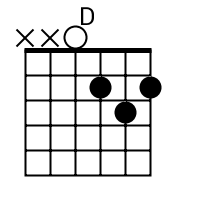
\includegraphics[width=3cm]{../Akordy/d.png}
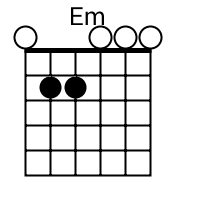
\includegraphics[width=3cm]{../Akordy/em.png}

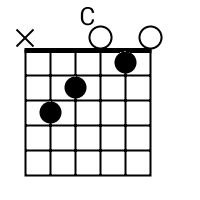
\includegraphics[width=3cm]{../Akordy/c.png}
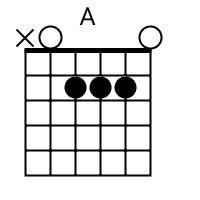
\includegraphics[width=3cm]{../Akordy/a.png}
	
\end{varwidth}

\end{centerjustified}
\setcounter{Slokočet}{0}
\end{song}
